\documentclass[11pt,a4paper]{article}
\usepackage[T1]{fontenc}
\usepackage[utf8]{inputenc}
\usepackage{lmodern,amsmath,amssymb,amsthm,graphicx,booktabs,array,microtype}
\usepackage[margin=25mm]{geometry}
\usepackage[font=small,labelfont=bf]{caption}
\usepackage[hidelinks]{hyperref}
\usepackage{float}
\usepackage{placeins}
\usepackage{fancyhdr}
\pagestyle{fancy}\fancyhf{}\fancyhead[L]{\small Energy-constrained deformation prediction}\fancyhead[R]{\small J. Fu}\fancyfoot[C]{\thepage}
\setlength{\headheight}{14pt}
\setlength{\parskip}{4pt}
\setlength{\parindent}{1.2em}
\setlength{\emergencystretch}{2em}
\newtheorem{proposition}{Proposition}
\newcommand{\dd}{\,\mathrm{d}}
\newcommand{\norm}[1]{\left\lVert #1\right\rVert}
\title{\textbf{Energy-Constrained Neural Surrogates for Large-Rotation Deformation of a Planar Flexible Finger}}
\author{Jiajun Fu\\\small Duke Kunshan University}
\date{October 2026}
\begin{document}
\maketitle
\begin{abstract}
Accurate deformation prediction under limited supervision is a central challenge in learning-based models of compliant structures. This paper examines whether a mechanical energy objective improves a neural load-to-shape surrogate for a planar flexible finger. The reference system is an inextensible Euler elastica with a spatially varying bending stiffness and a conservative transverse tip load. Supervised, energy-only, and hybrid models share a spectral rotation representation that exactly satisfies the clamped rotation and free-end moment conditions. The study uses 24 labeled equilibria, 256 unlabeled training parameters where required, and three initialization seeds. Each model is evaluated on 80 held-out cases in each of three regimes: interpolation, load extrapolation, and stiffness extrapolation. Reference solutions are verified against an independent continuous boundary-value solver, an analytical small-load limit, and a mesh-refinement study. Energy-only training reduces the mean load-extrapolation tip error from $0.548\%$ to $0.254\%$ of finger length, a reduction of $53.8\%$ relative to supervised training. The hybrid model attains the lowest mean errors for interpolation and stiffness extrapolation. A conditional continuum energy-error bound clarifies the relationship between potential-energy accuracy and geometric error. The findings support variational training within the examined reduced-order setting, while the fixed dataset and limited parameter family constrain broader conclusions.
\end{abstract}
\noindent\textbf{Keywords:} computational mechanics; physics-informed learning; nonlinear elastica; variational neural surrogate; soft robotics; out-of-distribution generalization.

\section{Introduction}
Compliant robotic components couple useful deformation with a modeling challenge: the relationship between loading and shape becomes nonlinear when rotations are large. Soft robotics provides a broader motivation for understanding and controlling such deformation \cite{rus2015}. A neural surrogate can approximate a parameter-to-equilibrium map, but sparse labeled data may leave that map poorly constrained away from observed configurations. Mechanical balance and kinematic admissibility offer additional structure for learning.

Physics-informed neural networks incorporate governing equations into statistical learning \cite{raissi2019}. Variational approaches instead train through an energy functional, as exemplified by the Deep Ritz method \cite{e2018} and deep energy methods for finite-deformation mechanics \cite{nguyen2020}. The two strategies share a physical motivation but impose different optimization problems. Their success depends on approximation, sampling, discretization, and optimization; incorporating physics does not by itself guarantee accurate prediction. Gradient pathologies and difficult optimization landscapes have been documented in physics-informed learning \cite{wang2021,krishnapriyan2021}.

This work considers a deliberately controlled question: \emph{with a shared mechanically admissible neural representation, how does replacing or supplementing sparse supervised training with a potential-energy objective affect deformation prediction under parameter extrapolation?} A planar cantilever with a two-parameter load and stiffness family permits independent numerical verification while retaining geometrically nonlinear kinematics. It is an idealized flexible finger, rather than a complete pneumatic or contact-driven gripper.

The study has three components. First, a parametric neural coefficient map is coupled to a rotation basis satisfying essential and natural boundary conditions. Second, supervised, energy-only, and hybrid objectives are compared under a common architecture and optimizer protocol. Third, reference verification and a conditional continuum error estimate provide a mechanical context for interpreting the empirical errors. The contribution is a focused computational comparison, rather than a new general-purpose neural mechanics method.

\section{Related work}
Physics-informed learning uses physical structure to constrain inference in forward and inverse problems \cite{raissi2019,karniadakis2021}. In strong-form approaches, differential-equation residuals are commonly evaluated at collocation points. For conservative mechanical systems, minimizing total potential energy provides an alternative that can avoid explicit evaluation of higher-order equilibrium derivatives. E and Yu developed the Deep Ritz formulation for variational problems \cite{e2018}; Nguyen-Thanh et al. applied a deep energy method to finite-deformation hyperelasticity \cite{nguyen2020}.

The present formulation differs in its approximation variable and target map. A neural network outputs coefficients of a finite rotation basis as a function of load and stiffness parameters. Spatial dependence is carried by that prescribed basis, rather than by a fully coordinate-based displacement network. It is therefore a finite-dimensional parametric surrogate. It does not establish discretization-invariant operator learning.

Studies of physics-informed optimization indicate that competing objective terms and difficult loss landscapes can affect convergence \cite{wang2021,krishnapriyan2021}. These observations motivate explicit reporting of optimization termination and a comparison within one shared architecture. Because all models below satisfy the same kinematic and boundary constraints, the experiments isolate the additional effect of variational training within that representation. They do not compare physical structure with an entirely unconstrained baseline.

\section{Mechanical model}
\subsection{Kinematics and nondimensionalization}
Consider a planar rod of length $L$, physical arclength $S\in[0,L]$, and bending stiffness $B(S)$. Let $B_0$ be a reference stiffness and $F$ a transverse force applied at the free end, with direction fixed in the laboratory frame. Introduce dimensionless variables
\begin{equation}
 s=\frac{S}{L},\qquad q=\frac{FL^2}{B_0},\qquad
 b(s)=\frac{B(Ls)}{B_0}=1+\alpha s,\qquad \alpha>-1.
 \label{eq:parameters}
\end{equation}
Here $\alpha$ controls the spatial gradient of bending stiffness. Positive and negative values represent increasing and decreasing stiffness, respectively; they do not uniquely specify a material composition or cross-section geometry.

Let $\theta(s)$ denote the tangent angle and $\mathbf r(s)=(x(s),y(s))$ the centerline divided by $L$. Inextensibility and an unshearable cross-section assumption yield
\begin{equation}
 \mathbf r'(s)=\begin{pmatrix}\cos\theta(s)\\\sin\theta(s)\end{pmatrix},
 \qquad \mathbf r(0)=\mathbf 0,\qquad \theta(0)=0.
 \label{eq:kinematics}
\end{equation}
The rod can undergo finite rotations, while its constitutive response remains linear in curvature. Extension, shear, inertia, self-contact, and viscoelasticity are excluded.

\subsection{Potential energy and equilibrium}
Dividing physical potential energy by $B_0/L$ gives
\begin{equation}
 \Pi[\theta;q,\alpha]
 =\frac12\int_0^1 b(s)\theta'(s)^2\dd s
 -q\int_0^1\sin\theta(s)\dd s.
 \label{eq:energy}
\end{equation}
The second term is $-q y(1)$, the potential of the conservative dead load. A follower force would require a different formulation. On the admissible space $V=\{v\in H^1(0,1):v(0)=0\}$, the first variation is
\begin{equation}
 \delta\Pi[\theta;\eta]
 =\int_0^1\left[b(s)\theta'(s)\eta'(s)-q\cos\theta(s)\eta(s)\right]\dd s,
 \qquad \eta\in V.
 \label{eq:variation}
\end{equation}
Integration by parts gives the nonlinear boundary-value problem
\begin{equation}
 (b\theta')'+q\cos\theta=0,\qquad
 \theta(0)=0,\qquad b(1)\theta'(1)=0.
 \label{eq:equilibrium}
\end{equation}
The free-end condition specifies zero bending moment. In the constant-stiffness, small-load limit,
\begin{equation}
 \theta(s)=q\left(s-\frac{s^2}{2}\right)+O(q^3),
 \qquad y(1)=\frac{q}{3}+O(q^3).
 \label{eq:smallload}
\end{equation}
This limit provides a reference-independent verification case.

\subsection{A sufficient energy-to-shape error bound}
The following estimate concerns the continuum functional and clarifies when energy accuracy controls geometric accuracy. It is a sufficient small-load condition, not a guarantee over the entire experimental domain.
\begin{proposition}
Let $b_{\min}=\min(1,1+\alpha)$ and
\begin{equation}
 \kappa=b_{\min}-\frac{4|q|}{\pi^2}>0.
 \label{eq:kappa}
\end{equation}
If $\theta_*\in V$ is a stationary solution of Eq.~\eqref{eq:energy}, then for every $\theta\in V$,
\begin{equation}
 \Pi[\theta]-\Pi[\theta_*]\geq
 \frac{\kappa}{2}\norm{\theta'-\theta_*'}_{L^2}^2,
 \label{eq:energybound}
\end{equation}
and the associated tip positions satisfy
\begin{equation}
 \norm{\mathbf r(1)-\mathbf r_*(1)}_2
 \leq\frac{2}{\pi}
 \sqrt{\frac{2\big(\Pi[\theta]-\Pi[\theta_*]\big)}{\kappa}}.
 \label{eq:tipbound}
\end{equation}
\end{proposition}
\begin{proof}
For $v\in V$, the one-ended Poincar\'e inequality gives $\norm{v}_{L^2}\leq(2/\pi)\norm{v'}_{L^2}$. Since $q\sin\theta\geq-|q|$,
\begin{equation}
 \delta^2\Pi[\theta](v,v)
 =\int_0^1\left[b(v')^2+q\sin\theta\,v^2\right]\dd s
 \geq\kappa\norm{v'}_{L^2}^2.
\end{equation}
Taylor's formula along the line from $\theta_*$ to $\theta$, together with stationarity, proves Eq.~\eqref{eq:energybound}. The unit-tangent map is 1-Lipschitz in its angle, so Eq.~\eqref{eq:kinematics} implies
$\norm{\mathbf r(1)-\mathbf r_*(1)}_2\leq\norm{\theta-\theta_*}_{L^1}\leq(2/\pi)\norm{\theta'-\theta_*'}_{L^2}$. Combining the inequalities establishes Eq.~\eqref{eq:tipbound}.
\end{proof}
The stiffness and load extrapolation tests include cases for which Eq.~\eqref{eq:kappa} is not satisfied. Moreover, the recorded discrete energy differences are not the continuum gaps in Eq.~\eqref{eq:tipbound}. The estimate is thus interpretive, rather than an a posteriori certificate for the reported predictions.

\section{Numerical and learning methods}
\subsection{Discrete reference solutions}
Let $s_i=ih$ for $i=0,\ldots,N$, with $h=1/N$ and $\theta_0=0$. Midpoint evaluation of stiffness and trapezoidal integration of the load potential give
\begin{equation}
 \Pi_h(\boldsymbol\theta;q,\alpha)
 =\frac{1}{2h}\sum_{i=1}^N b(s_{i-1/2})(\theta_i-\theta_{i-1})^2
 -q\sum_{i=0}^N w_i\sin\theta_i,
 \label{eq:discrete}
\end{equation}
where $w_0=w_N=h/2$ and $w_i=h$ otherwise. With $z_i=b(s_{i-1/2})(\theta_i-\theta_{i-1})/h$ and $z_{N+1}=0$, the derivative for a free degree of freedom is
\begin{equation}
 \frac{\partial\Pi_h}{\partial\theta_i}=z_i-z_{i+1}-q w_i\cos\theta_i,
 \qquad i=1,\ldots,N.
 \label{eq:gradient}
\end{equation}
Reference solutions use $N=256$ and L-BFGS-B minimization initialized with $q(s-s^2/2)/(1+\alpha/2)$. The iteration limit is 3,000, the relative objective tolerance is $10^{-14}$, and the projected-gradient tolerance is $10^{-8}$. The implementation rejects unsuccessful reference solves with an infinity-norm gradient above $2\times10^{-5}$. This initialization targets a low-energy bending branch; all stationary branches are not enumerated.

Centerlines are reconstructed by trapezoidal integration of Eq.~\eqref{eq:kinematics}. Reference angles are sampled at every fourth node to provide labels and evaluation values on the 64-segment prediction grid. An independent continuous solver uses the first-order system
\begin{equation}
 \theta'=\frac{m}{1+\alpha s},\qquad m'=-q\cos\theta,
 \qquad \theta(0)=0,\quad m(1)=0,
 \label{eq:bvp}
\end{equation}
where $m$ is dimensionless bending moment.

\subsection{Shared neural representation}
For parameters $\mathbf p=(q,\alpha)$, the neural angle is
\begin{equation}
 \theta_{\boldsymbol\omega}(s;\mathbf p)
 =\sum_{k=0}^{11} c_k(\mathbf p;\boldsymbol\omega)\phi_k(s),\qquad
 \phi_k(s)=\frac{\sin((k+\tfrac12)\pi s)}{(2k+1)^2}.
 \label{eq:basis}
\end{equation}
Every basis function satisfies $\phi_k(0)=0$ and $\phi_k'(1)=0$. Thus the clamp rotation and continuous free-end moment condition hold for every set of network weights. Integrating the unit tangent enforces continuum inextensibility; the plotted discrete centerline retains a quadrature error. The inverse-square frequency factor rescales coefficients to moderate optimization conditioning without changing the span of the 12 functions.

A fully connected network with dimensions $2$--$24$--$24$--$12$, tanh hidden activations, and a linear output maps $(q/1.5,\alpha/0.4)$ to the coefficients. It has 972 trainable parameters. Biases start at zero, and matrix entries are sampled independently from a centered normal distribution with standard deviation $0.35/\sqrt{n_{\mathrm{in}}}$. The same architecture, initialization seeds, and output basis are used for all objectives.

\subsection{Training objectives}
Let $\mathcal D_l$ contain $n_l=24$ labeled parameters with sampled reference angles, and let $\mathcal D_p$ contain $n_p=256$ independent unlabeled parameter samples. The supervised and energy objectives are
\begin{align}
 \mathcal L_d(\boldsymbol\omega)
 &=\frac{1}{n_lN}\sum_{\mathbf p\in\mathcal D_l}\sum_{i=1}^{N}
 \left|\theta_{\boldsymbol\omega}(s_i;\mathbf p)-\theta_{\mathrm{ref}}(s_i;\mathbf p)\right|^2,
 \label{eq:dataloss}\\
 \mathcal L_e(\boldsymbol\omega)
 &=\frac{1}{n_p}\sum_{\mathbf p\in\mathcal D_p}
 \Pi_h\big(\boldsymbol\theta_{\boldsymbol\omega}(\mathbf p);\mathbf p\big),\qquad N=64.
 \label{eq:energyloss}
\end{align}
The hybrid model minimizes
\begin{equation}
 \mathcal L_h=\mathcal L_e+0.1\mathcal L_d.
 \label{eq:hybridloss}
\end{equation}
The energy-only objective uses no reference labels. Its potentially negative value reflects the arbitrary energy origin and does not represent a negative prediction error. Separate sample means make the relative weighting independent of the two dataset sizes.

All models use explicit NumPy reverse-mode derivatives and full-batch L-BFGS-B, with a maximum of 1,800 iterations, relative objective tolerance $10^{-11}$, gradient tolerance $10^{-7}$, and memory parameter 30. The basis scaling and iteration budget were selected after an initial conditioning check. This protocol is an exploratory computational comparison, rather than a blinded hyperparameter-selection study.

\section{Experimental protocol and verification}
\subsection{Parameter domains and error measures}
Labeled and unlabeled parameters are drawn independently and uniformly from $[-1.5,1.5]\times[-0.4,0.4]$, using dataset seed 20261016. Three fixed test sets contain 80 cases each (Table~\ref{tab:domains}). Signs for extrapolation parameters are sampled with equal probability; magnitudes are uniform on the specified intervals. Initialization seeds are 0, 1, and 2. Test references do not enter any training objective.
\begin{table}[htbp]
 \centering\small
 \caption{Parameter domains. Each test set contains 80 cases.}\label{tab:domains}
 \begin{tabular}{lll}\toprule
 Dataset & Load $q$ & Stiffness gradient $\alpha$\\\midrule
 Training & $[-1.5,1.5]$ & $[-0.4,0.4]$\\
 Interpolation & $[-1.5,1.5]$ & $[-0.4,0.4]$\\
 Load extrapolation & $|q|\in[1.5,3]$ & $[-0.4,0.4]$\\
 Stiffness extrapolation & $[-1.5,1.5]$ & $|\alpha|\in[0.4,0.65]$\\\bottomrule
 \end{tabular}
\end{table}
For $M$ test parameters, the principal error is the average dimensionless tip distance,
\begin{equation}
 E_{\mathrm{tip}}=\frac1M\sum_{j=1}^M
 \norm{\mathbf r_{\boldsymbol\omega}(1;\mathbf p_j)-\mathbf r_{\mathrm{ref}}(1;\mathbf p_j)}_2.
 \label{eq:tipmetric}
\end{equation}
Secondary measures are the relative angle error $E_\theta$ and coordinate-wise centerline root-mean-square error $E_r$:
\begin{equation}
 E_\theta=\frac{\norm{\Theta_{\boldsymbol\omega}-\Theta_{\mathrm{ref}}}_F}{\norm{\Theta_{\mathrm{ref}}}_F},\qquad
 E_r=\frac{\norm{R_{\boldsymbol\omega}-R_{\mathrm{ref}}}_F}{\sqrt{2M(N+1)}}.
 \label{eq:secondary}
\end{equation}
Here $\Theta$ contains angles at the $N$ free nodes and $R$ contains both coordinates at $N+1$ nodes. Cross-seed sample standard deviations quantify initialization variability on one fixed dataset; they are not confidence intervals across independent data realizations.

\subsection{Verification of the reference and derivatives}
Five numerical tests check the discrete energy gradient, selected neural-network derivatives, the small-load analytical profile, load-sign symmetry and zero load, and reconstructed arclength. Finite differences validate the two gradient implementations. Reference agreement with Eq.~\eqref{eq:bvp} is assessed at three nonlinear cases using adaptive collocation with tolerance $10^{-9}$ (Table~\ref{tab:bvp}).
\begin{table}[htbp]
\centering\small
\caption{Maximum nodal angle difference between the 256-segment reference and the independent continuous boundary-value solver.}\label{tab:bvp}
\begin{tabular}{rrc}\toprule
$q$ & $\alpha$ & Maximum difference (rad)\\\midrule
1 & 0 & $3.153\times 10^{-7}$\\
3 & -0.4 & $5.726\times 10^{-7}$\\
-2 & 0.6 & $2.413\times 10^{-6}$\\
\bottomrule\end{tabular}
\end{table}

A separate refinement study at $(q,\alpha)=(3,-0.4)$ uses 16--512 segments (Fig.~\ref{fig:convergence}). The change in tip position from 256 to 512 segments is $1.928\times10^{-6}$ finger lengths. This check suggests that reference discretization error is small relative to the reported mean tip errors at the examined refinement case, but does not establish a uniform bound over all parameter values.
\begin{figure}[htbp]
 \centering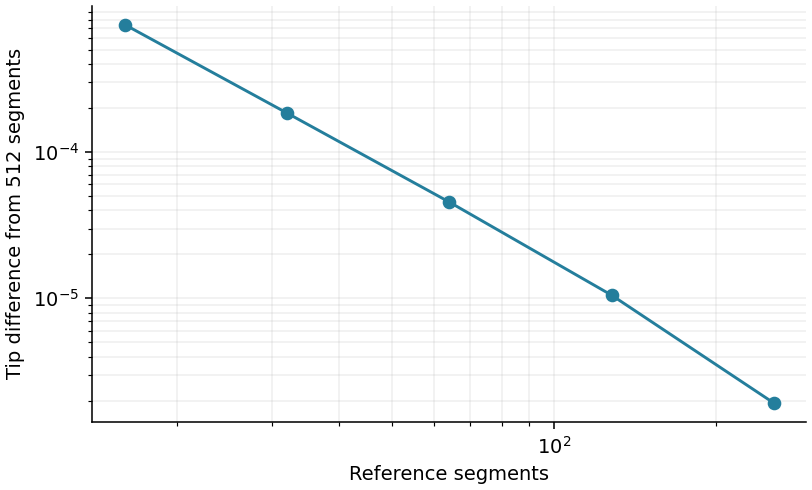
\includegraphics[width=0.68\textwidth]{../figures/convergence.png}
 \caption{Reference tip convergence at $q=3$, $\alpha=-0.4$. Differences are measured against the 512-segment solution, which is a numerical comparison rather than an exact solution.}\label{fig:convergence}
\end{figure}

\section{Results}
\subsection{Tip prediction under interpolation and extrapolation}
Table~\ref{tab:tip} summarizes the mean tip errors. The hybrid model yields the lowest interpolation error, $8.07\times10^{-5}$, compared with $3.54\times10^{-4}$ for supervised training. Under load extrapolation, the energy-only model attains $2.54\times10^{-3}$, compared with $5.48\times10^{-3}$ for the supervised model and $2.77\times10^{-3}$ for the hybrid model. The hybrid model gives the lowest stiffness-extrapolation error, $9.15\times10^{-4}$, compared with $3.11\times10^{-3}$ for supervised training.
\begin{table}[htbp]
\centering\small
\caption{Tip error in units of $10^{-3}$ finger lengths: mean $\pm$ sample standard deviation across three initialization seeds. Each seed is evaluated on the same 80 test cases per split.}\label{tab:tip}
\begin{tabular}{lccc}\toprule
Test regime & Supervised & Energy only & Hybrid\\\midrule
Interpolation & $0.354 \pm 0.108$ & $0.089 \pm 0.003$ & $0.081 \pm 0.017$\\
Load extrapolation & $5.482 \pm 2.136$ & $2.535 \pm 1.356$ & $2.765 \pm 1.112$\\
Stiffness extrapolation & $3.106 \pm 1.276$ & $1.003 \pm 0.233$ & $0.915 \pm 0.272$\\
\bottomrule\end{tabular}
\end{table}

The corresponding reductions relative to the supervised mean are approximately $77.2\%$ for hybrid interpolation, $53.8\%$ for energy-only load extrapolation, and $70.5\%$ for hybrid stiffness extrapolation. These percentages are descriptive comparisons on the fixed test sets. With only three initialization seeds and one data realization, they do not establish population-level statistical significance.
\begin{figure}[htbp]
 \centering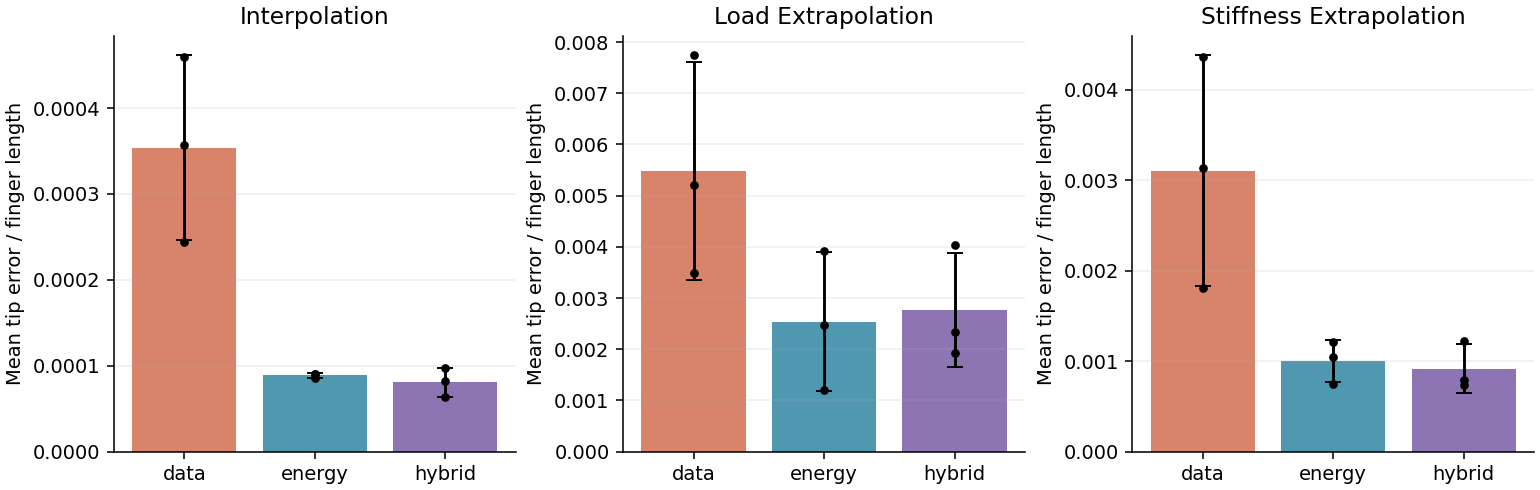
\includegraphics[width=\textwidth]{../figures/benchmark.png}
 \caption{Tip errors for the three test regimes. Bars denote means across initialization seeds, error bars denote sample standard deviations, and points show individual runs. All methods share the same mechanically admissible representation.}\label{fig:benchmark}
\end{figure}
Figure~\ref{fig:benchmark} shows that initialization sensitivity is more pronounced outside the training domain. For load extrapolation, the standard deviation is $2.14\times10^{-3}$ for supervised training and $1.36\times10^{-3}$ for energy-only training. The energy and hybrid means are close relative to their cross-seed variation, so their numerical ranking should not be interpreted as a decisive separation.

\subsection{Rotation and centerline accuracy}
The secondary measures show a similar pattern (Table~\ref{tab:secondary}). For load extrapolation, energy-only training reduces mean relative angle error from approximately $1.25\times10^{-2}$ to $8.13\times10^{-3}$ and mean coordinate-wise centerline RMSE from $2.67\times10^{-3}$ to $1.18\times10^{-3}$. Thus the improvement is not limited to cancellation at the tip. The different metrics need not produce identical rankings because they weight field errors differently.
\begin{table}[htbp]
\centering\small
\caption{Mean relative angle error $E_\theta$ and coordinate-wise centerline RMSE $E_r$, averaged across initialization seeds. Both columns are expressed in units of $10^{-3}$.}\label{tab:secondary}
\begin{tabular}{llrr}\toprule
Test regime & Method & $10^3 E_\theta$ & $10^3 E_r$\\\midrule
Interpolation & Supervised & 2.549 & 0.184\\
 & Energy only & 0.630 & 0.039\\
 & Hybrid & 0.577 & 0.037\\
\midrule
Load extrapolation & Supervised & 12.516 & 2.673\\
 & Energy only & 8.126 & 1.177\\
 & Hybrid & 8.310 & 1.200\\
\midrule
Stiffness extrapolation & Supervised & 17.864 & 1.165\\
 & Energy only & 7.065 & 0.373\\
 & Hybrid & 6.543 & 0.357\\
\bottomrule\end{tabular}
\end{table}

\begin{figure}[htbp]
 \centering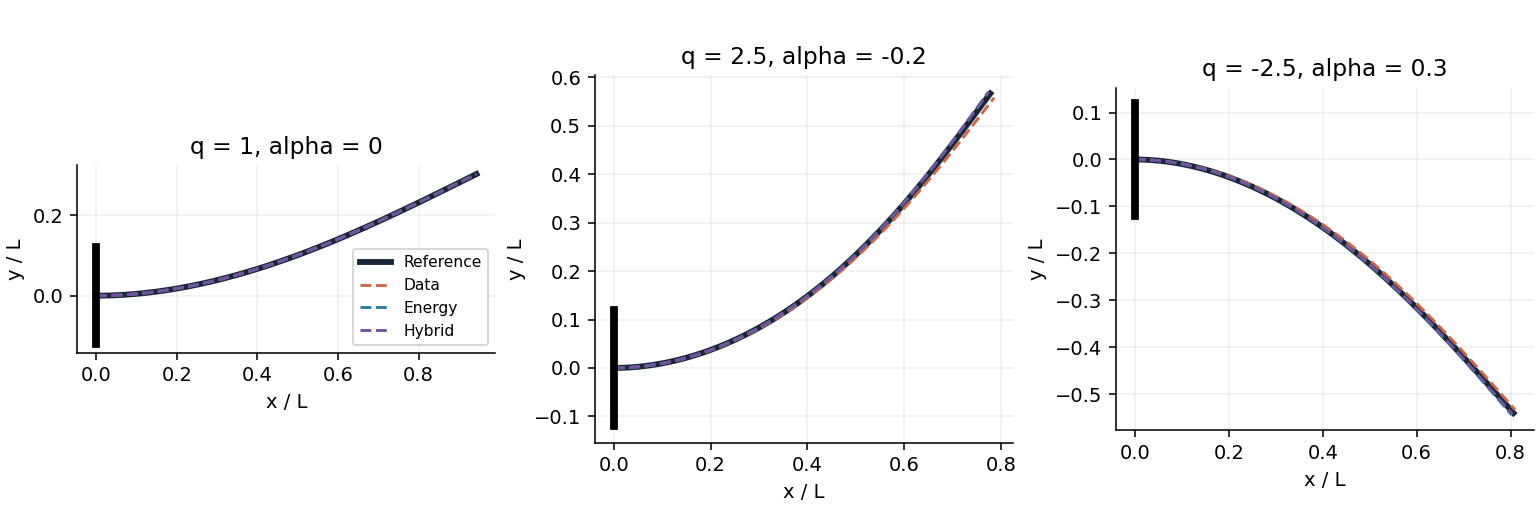
\includegraphics[width=\textwidth]{../figures/shapes.png}
 \caption{Centerlines for initialization seed 0 at three representative parameter values. The first case lies within the training domain; the other two have load magnitudes beyond the training interval. Curves are shown at their actual dimensionless coordinates.}\label{fig:shapes}
\end{figure}
The representative shapes in Fig.~\ref{fig:shapes} illustrate agreement in the gross bending response. Visual overlap alone cannot resolve the small errors reported in the tables, and these selected configurations are not a substitute for evaluation over the full test sets.

\subsection{Optimization and energy diagnostics}
Six of the nine training runs satisfy the optimizer's relative-objective stopping criterion. The energy-only seed-0 run and hybrid seed-0 and seed-2 runs reach the 1,800-iteration budget. Final weight-gradient infinity norms range from $7.63\times10^{-7}$ to $5.87\times10^{-6}$. Reported predictions include all runs; the iteration-limited models are not discarded. Since each iteration evaluates different objectives, equal iteration limits do not imply equal computational costs.

On the load-extrapolation set, mean discrete energy gaps relative to sampled reference angles decrease from $3.17\times10^{-4}$ for supervised learning to $1.31\times10^{-4}$ for energy-only learning and $1.16\times10^{-4}$ for the hybrid model. The hybrid energy gap is smaller even though its mean tip error is slightly larger than that of the energy-only model. Energy gaps and geometric errors therefore provide complementary information. In particular, the continuum estimate in Eq.~\eqref{eq:tipbound} cannot be applied directly to these discrete gaps outside its stated parameter regime.

\subsection{Quasistatic continuation visualizations}
Supplementary animations evaluate a load path $q=2.8\sin\tau$ at $\alpha=-0.2$ and a stiffness path $\alpha\in[-0.65,0.65]$ at $q=1.3$. Each frame is an independently computed equilibrium; $\tau$ is a visualization parameter rather than physical time. Figure~\ref{fig:sweep} shows one frame of the load path together with tip-error curves. These visualizations illustrate shape response and extrapolation without introducing an unmodeled dynamical interpretation.
\begin{figure}[htbp]
 \centering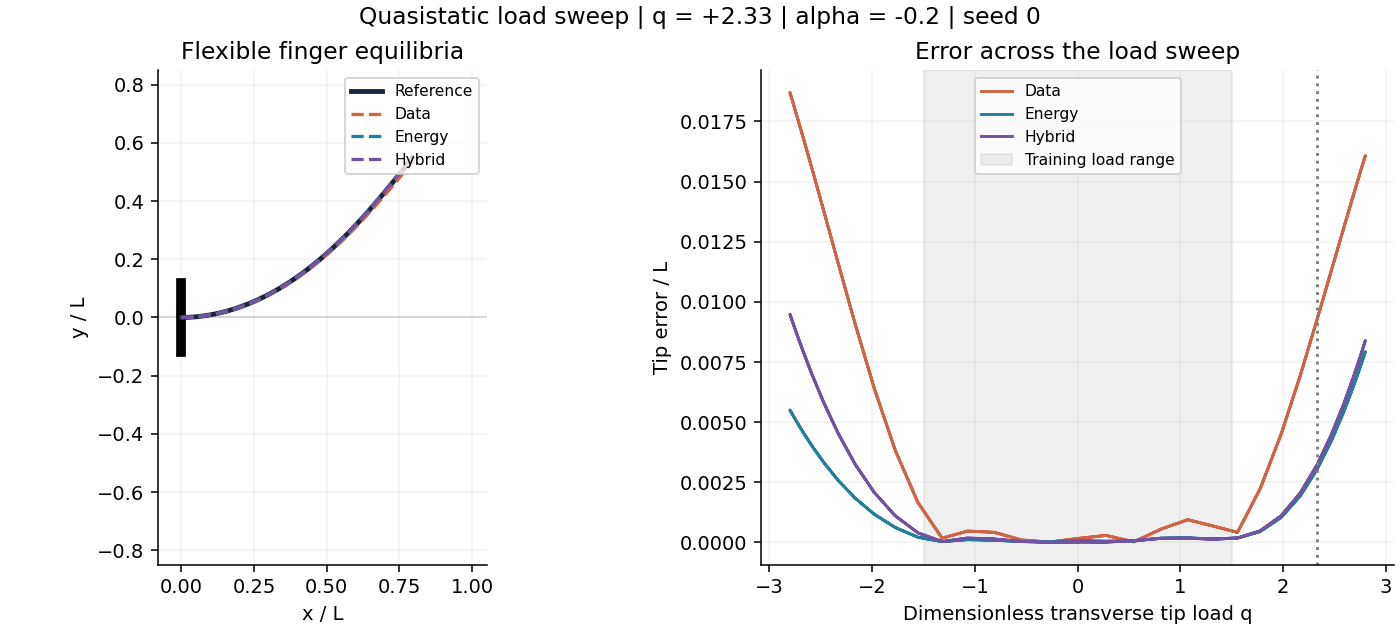
\includegraphics[width=0.94\textwidth]{../figures/animation_still.png}
 \caption{Load-path visualization for seed 0. The shaded interval marks training loads. The left panel compares equilibrium shapes; the right panel shows tip error over the path.}\label{fig:sweep}
\end{figure}
\FloatBarrier

\section{Discussion}
\subsection{Interpretation of the variational objective}
The energy-only model obtains lower mean errors than supervised learning across all three test regimes despite using no reference labels. This finding indicates that the sampled mechanical functional supplies useful information about the parameter-to-shape map within this two-parameter rod family. In the hybrid formulation, the small supervised term further improves mean interpolation and stiffness extrapolation, while offering no mean advantage over energy-only training for load extrapolation.

The comparison should be interpreted in light of the shared representation. Every model satisfies the same clamp, free-end moment condition, and continuum inextensibility. The supervised baseline is already mechanically structured. The observed differences concern the additional energy objective and unlabeled parameter samples, rather than the value of physics in general. Likewise, because the supervised model uses 24 labeled cases while the variational models use 256 additional parameter samples, this is a comparison under different information sources, not a matched-sample or matched-compute experiment.

The analytical estimate separates a useful principle from the numerical evidence: in a sufficient coercive regime, an energy gap controls a rotation-gradient error and, consequently, tip error. At larger loads the sufficient condition can fail, and finite sampling of the parameter space does not enforce equilibrium at unseen parameters. The empirical extrapolation improvement is therefore a measured property of the trained surrogates, not a consequence guaranteed throughout the test domain by the proposition.

\subsection{Limitations}
The mechanical model is one-dimensional, inextensible, quasistatic, and planar. It does not include pressure actuation, volumetric constitutive response, shear, contact, material hysteresis, or three-dimensional motion. The stiffness family is affine in arclength and has only one variation parameter. Conclusions cannot be transferred directly to arbitrary soft grippers or heterogeneous solids.

The experiment uses one dataset seed, three initialization seeds, one label count, and one hybrid loss weight. The initial conditioning check informed representation scaling and the training budget; a separate validation-based selection procedure was not conducted. Twelve basis modes and a 64-segment quadrature grid limit approximation and energy resolution. A convergence study of the neural representation, label-count sensitivity, and loss-weight sensitivity remains necessary for broader methodological claims.

Reference verification covers three continuous-solver comparisons and one refinement path. Optimization follows an initialized low-energy branch without classifying every equilibrium or certifying global minimality. In addition, three training runs reach the prescribed budget. These restrictions motivate interpreting the results as a reproducible computational study of one controlled system. No experimental validation or general inference-time speedup is asserted.

\section{Conclusion}
A mechanically admissible parametric neural surrogate was evaluated for the large-rotation deformation of a planar flexible finger. Against a supervised model with the same architecture, minimum-potential-energy training reduced mean load-extrapolation tip error by $53.8\%$ on the specified test set. Hybrid training achieved the lowest mean interpolation and stiffness-extrapolation errors. Independent solver checks, analytical verification, and mesh refinement support the numerical reference, while a sufficient continuum bound explains a restricted relationship between energy and shape accuracy.

The results support further investigation of variational learning for reduced compliant-structure models. Priority extensions are independent dataset repetitions, systematic label and loss-weight studies, basis and quadrature refinement, and a verified two-dimensional hyperelastic reference model. Pressure actuation and contact should be introduced only after the corresponding mechanics and numerical solvers are independently validated.

\section*{Data and code availability}
All data are synthetic. Source code, saved weights, test parameters, numerical verification results, and supplementary animations are available at \url{https://github.com/Fjj040806/Physically-Constrained-Deformation-Prediction}. Dataset and initialization seeds, optimizer histories, and dependency versions are included for reproduction. No external experimental dataset is used.

\section*{Disclosure of AI assistance}
AI tools assisted with implementation, numerical analysis, and manuscript drafting. The manuscript reports the computations contained in the accompanying repository.

\begin{thebibliography}{9}
\bibitem{rus2015} D. Rus and M. T. Tolley, ``Design, fabrication and control of soft robots,'' \emph{Nature}, vol. 521, pp. 467--475, 2015. \href{https://doi.org/10.1038/nature14543}{doi:10.1038/nature14543}.
\bibitem{raissi2019} M. Raissi, P. Perdikaris, and G. E. Karniadakis, ``Physics-informed neural networks: A deep learning framework for solving forward and inverse problems involving nonlinear partial differential equations,'' \emph{Journal of Computational Physics}, vol. 378, pp. 686--707, 2019. \href{https://doi.org/10.1016/j.jcp.2018.10.045}{doi:10.1016/j.jcp.2018.10.045}.
\bibitem{e2018} W. E and B. Yu, ``The Deep Ritz method: A deep learning-based numerical algorithm for solving variational problems,'' \emph{Communications in Mathematics and Statistics}, vol. 6, pp. 1--12, 2018. \href{https://doi.org/10.1007/s40304-018-0127-z}{doi:10.1007/s40304-018-0127-z}.
\bibitem{nguyen2020} V. M. Nguyen-Thanh, X. Zhuang, and T. Rabczuk, ``A deep energy method for finite deformation hyperelasticity,'' \emph{European Journal of Mechanics--A/Solids}, vol. 80, article 103874, 2020. \href{https://doi.org/10.1016/j.euromechsol.2019.103874}{doi:10.1016/j.euromechsol.2019.103874}.
\bibitem{wang2021} S. Wang, Y. Teng, and P. Perdikaris, ``Understanding and mitigating gradient flow pathologies in physics-informed neural networks,'' \emph{SIAM Journal on Scientific Computing}, vol. 43, no. 5, 2021. \href{https://doi.org/10.1137/20M1318043}{doi:10.1137/20M1318043}.
\bibitem{krishnapriyan2021} A. Krishnapriyan, A. Gholami, S. Zhe, R. M. Kirby, and M. W. Mahoney, ``Characterizing possible failure modes in physics-informed neural networks,'' \emph{Advances in Neural Information Processing Systems}, vol. 34, 2021. \url{https://arxiv.org/abs/2109.01050}.
\bibitem{karniadakis2021} G. E. Karniadakis et al., ``Physics-informed machine learning,'' \emph{Nature Reviews Physics}, vol. 3, pp. 422--440, 2021. \href{https://doi.org/10.1038/s42254-021-00314-5}{doi:10.1038/s42254-021-00314-5}.
\end{thebibliography}
\end{document}
